\documentclass{beamer}

\usepackage{amssymb,amsmath}
\usepackage{graphicx}
\usepackage{url}
\usepackage{color}
\usepackage{pagenote}[continuous,page]
\usepackage{relsize}		% For \smaller
\usepackage{url}			% For \url
\usepackage{epstopdf}	% Included EPS files automatically converted to PDF to include with pdflatex

%For MindMaps
% \usepackage{tikz}%
% \usetikzlibrary{mindmap,trees,arrows}%

%%% Color Definitions %%%%%%%%%%%%%%%%%%%%%%%%%%%%%%%%%%%%%%%%%%%%%%%%%%%%%%%%%
%\definecolor{bordercol}{RGB}{40,40,40}
%\definecolor{headercol1}{RGB}{186,215,230}
%\definecolor{headercol2}{RGB}{80,80,80}
%\definecolor{headerfontcol}{RGB}{0,0,0}
%\definecolor{boxcolor}{RGB}{186,215,230}

%%% Save space in lists. Use this after the opening of the list %%%%%%%%%%%%%%%%
%\newcommand{\compresslist}{
%	\setlength{\itemsep}{1pt}
%	\setlength{\parskip}{0pt}
%	\setlength{\parsep}{0pt}
%}

%\setbeameroption{show notes on top}

% You should run 'pdflatex' TWICE, because of TOC issues.

% Rename this file.  A common temptation for first-time slide makers
% is to name it something like ``my_talk.tex'' or
% ``john_doe_talk.tex'' or even ``discrete_math_seminar_talk.tex''.
% You really won't like any of these titles the second time you give a
% talk.  Try naming your tex file something more descriptive, like
% ``riemann_hypothesis_short_proof_talk.tex''.  Even better (in case
% you recycle 99% of a talk, but still want to change a little, and
% retain copies of each), how about
% ``riemann_hypothesis_short_proof_MIT-Colloquium.2000-01-01.tex''?

\mode<presentation>
{
  \usetheme{CambridgeUS}		% bem bacana - menu superior
  \usecolortheme{default}		% branco, azul clarinho
  \useoutertheme{default}
  \useinnertheme{circles}
  \setbeamercovered{invisible}
}

\beamertemplatenavigationsymbolsempty

%% Better looking blocks
\setbeamercolor{block title alerted}{use=structure,fg=black,bg=red!80!black}
\setbeamercolor{block body alerted}{use=structure,fg=black,bg=white!90!black}

\setbeamercolor{block title}{use=structure,fg=black,bg=blue!60!white}
\setbeamercolor{block body}{use=structure,fg=black,bg=white!90!black}

\usepackage[english]{babel}
\usepackage[latin1]{inputenc}
\usepackage{subfigure}

\usepackage{times}
\usepackage[T1]{fontenc}

%% makes the ppagenote command for figure references at the end.
\makepagenote
\renewcommand{\notenumintext}[1]{}
\newcommand{\ppagenote}[1]{\pagenote[Page \insertframenumber]{#1}}


\usepackage{tikz}
\usetikzlibrary{arrows,shapes}

\title[GB13604]{GB13604 - Maths for Computer Science}
\subtitle[]{Lecture 5 -- Graphs Part II}
\author[Claus Aranha]{Claus Aranha\\{\footnotesize caranha@cs.tsukuba.ac.jp}}
\institute[COINS]{College of Information Science}
\date[2018-11-07]{2018-11-07\\{\tiny Last updated \today}}

\tikzstyle{vertex}=[circle,fill=black!25,minimum size=10pt,inner sep=0pt]
\tikzstyle{blue vertex}=[circle,fill=blue!100,minimum size=10pt,inner sep=0pt]
\tikzstyle{red vertex}=[circle,fill=red!100,minimum size=10pt,inner sep=0pt]
\tikzstyle{yellow vertex}=[circle,fill=yellow!100,minimum size=10pt,inner sep=0pt]
\tikzstyle{edge} = [draw,thick,-]
\tikzstyle{pedge} = [draw,thick,.]
\tikzstyle{red edge} = [draw, thick,-,red!50]
\tikzstyle{black edge} = [draw, line width=2pt,-,black!20]
\tikzstyle{weight} = [font=\smaller]

\begin{document}

\begin{frame}
  \maketitle

  \begin{center}
    {\smaller This course is based on Mathematics for Computer Science, Spring
    2015, by Albert Meyer and Adam Chlipala, Massachusetts Institute
    of Technology OpenCourseWare.}
    
    
\includegraphics[width=0.2\textwidth]{../img/by-nc-sa}
  \end{center}
\end{frame}

\section{Introduction}

\begin{frame}
  \frametitle{Exercise Discussion, Weeks 3 and 4}

\end{frame}

\begin{frame}
  \frametitle{Week 4 and 5 summary}

  {\larger
    {\bf Graphs}

    \bigskip

    \begin{center}
      Lecture I: Chapter 9
    \end{center}
    \begin{itemize}
    \item Walks and Paths
    \item Scheduling and Partial Orders
    \item Equivalence Relations

      \bigskip

      \begin{center}
        Lecture II: Chapter 11
      \end{center}
    \item Isomorphism
    \item Coloring and Connectivity
    \item Spanning Trees
    \item Matching
    \end{itemize}
  }
\end{frame}

\section{Degrees and Ismorphism}
\begin{frame}
  \frametitle{Simple Graphs and Directed Graphs}

  {\larger
  \begin{columns}[T]
    \column{0.5\textwidth}
    \begin{center}
      Directed Graph:\\
      
      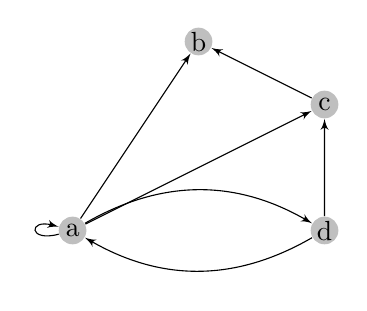
\begin{tikzpicture}[scale=.8,auto,swap]
        \tikzset{edge/.style = {->,>=latex'}}
        \node[vertex] (a) at (0,0) {a};
        \node[vertex] (b) at (2,3) {b};
        \node[vertex] (c) at (4,2) {c};
        \node[vertex] (d) at (4,0) {d};
        \draw[edge] (a) to (b);
        \draw[edge] (a) to (c);
        \draw[edge] (c) to (b);
        \draw[edge] (d) to (c);
        \draw[edge] (d) to[bend left] (a);
        \draw[edge] (a) to[bend left] (d);
        \draw[edge] (a) to[loop left] (a);
      \end{tikzpicture}
    \end{center}
    \column{0.5\textwidth}
    \begin{center}
      Simple Graph:\\
      
      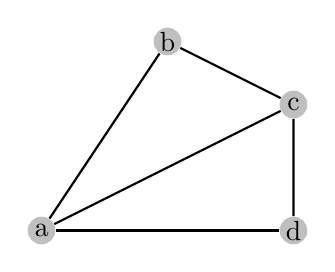
\begin{tikzpicture}[scale=.8,auto,swap]
        %\tikzset{edge/.style = {->,>=latex'}}
        \node[vertex] (a) at (0,0) {a};
        \node[vertex] (b) at (2,3) {b};
        \node[vertex] (c) at (4,2) {c};
        \node[vertex] (d) at (4,0) {d};
        \draw[edge] (a) to (b);
        \draw[edge] (a) to (c);
        \draw[edge] (c) to (b);
        \draw[edge] (d) to (c);
        \draw[edge] (d) to (a);
      \end{tikzpicture}

      \vspace{2em}      
    \end{center}
    \begin{itemize}
    \item No double edges allowed;
    \item No self-loop allowed;
    \end{itemize}
  \end{columns}
  }
\end{frame}

\begin{frame}
  \frametitle{Simple Graphs: Formal definitions}

  {\larger
    A Simple Graph \structure{$G$} consists of:
    \begin{itemize}
    \item A non-empty set \structure{$V$} of vertices;
    \item A set \structure{$E$} of edges so that:
      \begin{itemize}
      \item Each edge has \structure{two endpoints} in $V$\\
        \hfill (\alert{not an {\bf start} and an {\bf end}})

        \bigskip
      \item The order of the vertices do not matter\\
        \hfill $e_1 = \{v_1,v_2\} = \{v_2, v_1\}$

        \bigskip
      \item Two vertices with an edge between them are
        \structure{adjacent}

        \bigskip
      \item An edge that connects two vertices is \structure{incident}
        to them.\\
        \hfill ($e_1$ is \structure{incident} to $v_1$ and $v_2$)
      \end{itemize}
    \end{itemize}
  }
\end{frame}

\begin{frame}
  \frametitle{The Degree of a Vertex}

  {\larger

    The \structure{degree} of a vertex is the \structure{number of
      incident edges}.

    \begin{center}
      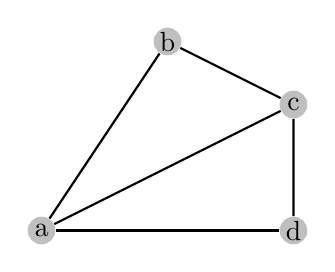
\begin{tikzpicture}[scale=.8,auto,swap]
        %\tikzset{edge/.style = {->,>=latex'}}
        \node[vertex] (a) at (0,0) {a};
        \node[vertex] (b) at (2,3) {b};
        \node[vertex] (c) at (4,2) {c};
        \node[vertex] (d) at (4,0) {d};
        \draw[edge] (a) to (b);
        \draw[edge] (a) to (c);
        \draw[edge] (c) to (b);
        \draw[edge] (d) to (c);
        \draw[edge] (d) to (a);
      \end{tikzpicture}

      deg(a) = 3 \hspace{1cm} deg(d) = 2
    \end{center}

    \hfill

    \alert{Quiz:} Is there a graph with degrees:
    \begin{itemize}
    \item 2, 2, 1?
    \item 3, 2, 2, 1?
    \end{itemize}
  }
\end{frame}

\begin{frame}
  \frametitle{Degree Properties}

  {\larger
    
    \structure{The Handshaking Lemma:}\\
    \hspace{1cm}The sum of degrees must be 2x the number of edges
    \begin{equation}
      2|E| = \sum_{v\in V} \text{deg}(v)
    \end{equation}
    \hfill{\bf Proof:} Each edge contribute 2 to LHS of (1)

    \bigskip

    So ``2 + 2 + 1 = odd'' is impossible!
    }
\end{frame}

\subsection{Isomorphism}

\begin{frame}
  \frametitle{Isomorphism: The Graph Abstraction}

  {\larger
    \begin{columns}
      \column{0.5\textwidth}
      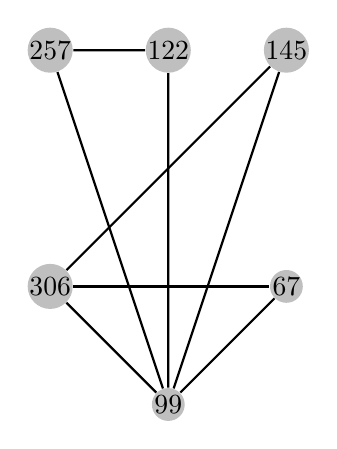
\begin{tikzpicture}[scale=1.5,auto,swap]
        %\tikzset{edge/.style = {->,>=latex'}}
        \node[vertex] (257) at (0,2) {257};
        \node[vertex] (122) at (1,2) {122};
        \node[vertex] (145) at (2,2) {145};
        \node[vertex] (306) at (0,0) {306};
        \node[vertex] (67) at (2,0) {67};
        \node[vertex] (99) at (1,-1) {99};
        \draw[edge] (257) to (122);
        \draw[edge] (257) to (99);
        \draw[edge] (122) to (99);
        \draw[edge] (306) to (99);
        \draw[edge] (67) to (99);
        \draw[edge] (306) to (67);
        \draw[edge] (306) to (145);
        \draw[edge] (145) to (99);
      \end{tikzpicture}
      
      \column{0.5\textwidth}
      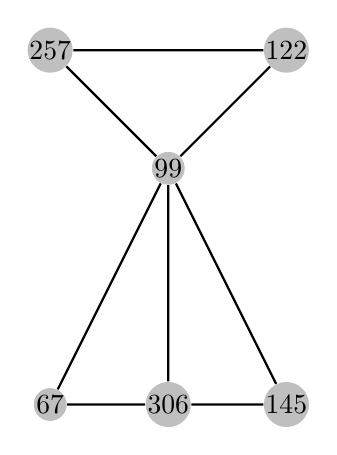
\begin{tikzpicture}[scale=1.5,auto,swap]
        %\tikzset{edge/.style = {->,>=latex'}}
        \node[vertex] (257) at (0,2) {257};
        \node[vertex] (122) at (2,2) {122};
        \node[vertex] (145) at (2,-1) {145};
        \node[vertex] (306) at (1,-1) {306};
        \node[vertex] (67) at (0,-1) {67};
        \node[vertex] (99) at (1,1) {99};
        \draw[edge] (257) to (122);
        \draw[edge] (257) to (99);
        \draw[edge] (122) to (99);
        \draw[edge] (306) to (99);
        \draw[edge] (67) to (99);
        \draw[edge] (306) to (67);
        \draw[edge] (306) to (145);
        \draw[edge] (145) to (99);
      \end{tikzpicture}
      
    \end{columns}

    \bigskip

    \structure{Same Graph}, \alert{Different Layouts}
  }
\end{frame}

\begin{frame}
  \frametitle{Isomorphism: The Graph Abstraction}

  {\larger
    \begin{columns}
      \column{0.5\textwidth}
      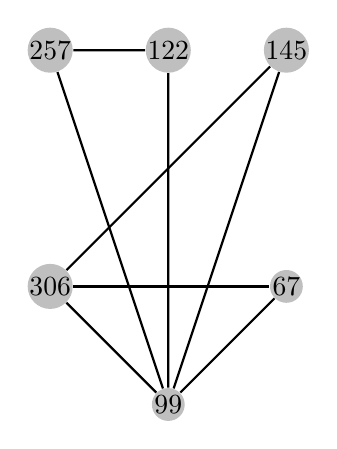
\begin{tikzpicture}[scale=1.5,auto,swap]
        %\tikzset{edge/.style = {->,>=latex'}}
        \node[vertex] (257) at (0,2) {257};
        \node[vertex] (122) at (1,2) {122};
        \node[vertex] (145) at (2,2) {145};
        \node[vertex] (306) at (0,0) {306};
        \node[vertex] (67) at (2,0) {67};
        \node[vertex] (99) at (1,-1) {99};
        \draw[edge] (257) to (122);
        \draw[edge] (257) to (99);
        \draw[edge] (122) to (99);
        \draw[edge] (306) to (99);
        \draw[edge] (67) to (99);
        \draw[edge] (306) to (67);
        \draw[edge] (306) to (145);
        \draw[edge] (145) to (99);
      \end{tikzpicture}
      
      \column{0.5\textwidth}
      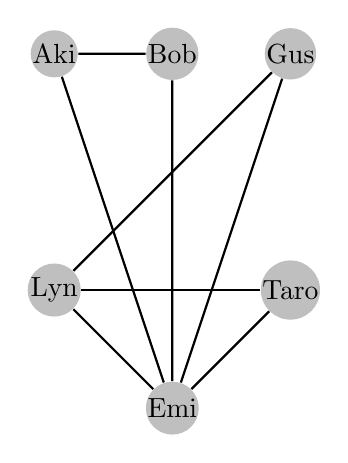
\begin{tikzpicture}[scale=1.5,auto,swap]
        %\tikzset{edge/.style = {->,>=latex'}}
        \node[vertex] (257) at (0,2) {Aki};
        \node[vertex] (122) at (1,2) {Bob};
        \node[vertex] (145) at (2,2) {Gus};
        \node[vertex] (306) at (0,0) {Lyn};
        \node[vertex] (67) at (2,0) {Taro};
        \node[vertex] (99) at (1,-1) {Emi};
        \draw[edge] (257) to (122);
        \draw[edge] (257) to (99);
        \draw[edge] (122) to (99);
        \draw[edge] (306) to (99);
        \draw[edge] (67) to (99);
        \draw[edge] (306) to (67);
        \draw[edge] (306) to (145);
        \draw[edge] (145) to (99);
      \end{tikzpicture}
      
    \end{columns}

    \bigskip

    \structure{Same Graph}, \alert{Different Labels}\\
    \hfill {\bf Isomorphic Graphs}
  }
\end{frame}

\begin{frame}
  \frametitle{Isomorphic Graphs}

  {\larger
    \begin{itemize}
    \item To determine \structure{isomorphism}, all that matters is connections;

      \bigskip
      
    \item Graphs with the same connections are \structure{isomorphic}

      \vfill
      
    \item Two graphs are isomorphic if there is a \structure{Edge
      Preserving Matching} of their vertices.\\
      \hfill ...In other words, a {\bf bijection} between the vertices.
    \end{itemize}
  }
\end{frame}

\begin{frame}
  \frametitle{Are these Graphs Isomorphic?}

    {\larger
    \begin{columns}
      \column{0.5\textwidth}
      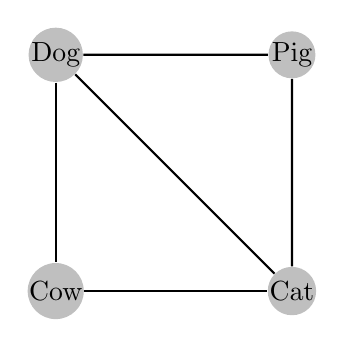
\begin{tikzpicture}[scale=1.5,auto,swap]
        %\tikzset{edge/.style = {->,>=latex'}}
        \node[vertex] (a) at (0,0) {Cow};
        \node[vertex] (b) at (2,0) {Cat};
        \node[vertex] (c) at (0,2) {Dog};
        \node[vertex] (d) at (2,2) {Pig};
        \draw[edge] (a) to (b);
        \draw[edge] (b) to (d);
        \draw[edge] (d) to (c);
        \draw[edge] (c) to (a);
        \draw[edge] (c) to (b);
      \end{tikzpicture}
      \column{0.5\textwidth}
      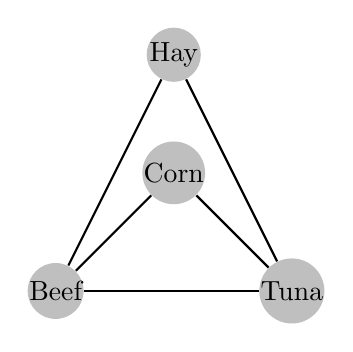
\begin{tikzpicture}[scale=1.5,auto,swap]
        %\tikzset{edge/.style = {->,>=latex'}}
        \node[vertex] (a) at (1,2) {Hay};
        \node[vertex] (b) at (2,0) {Tuna};
        \node[vertex] (c) at (0,0) {Beef};
        \node[vertex] (d) at (1,1) {Corn};
        \draw[edge] (a) to (b);
        \draw[edge] (b) to (d);
        \draw[edge] (d) to (c);
        \draw[edge] (c) to (a);
        \draw[edge] (c) to (b);
      \end{tikzpicture}
    \end{columns}

    \bigskip
    f(dog) = Beef; \hspace{2cm} f(cow) = Hay\\
    f(cat) = Tuna; \hspace{2cm} f(pig) = Corn

    \bigskip

    Is this a Bijection? Are the Edges preserved?
    }
\end{frame}

\begin{frame}
  \frametitle{Formal Definition of Graph Isomorphism}

  {\larger
    $G_1$ \structure{isomorphic} to $G_2$ means that $\exists$
    Edge Preserving Vertex Matching:
    \begin{equation}
      \exists f:V_1 \rightarrow V_2, 
      (u,v) \in E_1 \iff (f(u),f(v)) \in E_2
    \end{equation}

    \bigskip

    Two graphs are \alert{non}isomorphic if:
    \begin{itemize}
    \item Not the same number of vertices;
    \item Not the same number of edges;
    \item Not the same degree distribution;
    \item Differenes in Paths, Distances, etc...
    \end{itemize}
  }
\end{frame}

\begin{frame}
  \frametitle{Finding Isomorphism}

  {\larger
    \begin{itemize}
    \item Small Graphs: Check properties by hand;
    \item Large Graphs: Search for a {\bf matching $f: V_1 \rightarrow V_2$}
      that \structure{Preserve~Isomorphic~Properties}:
      \begin{itemize}
      \item Check vertices with \alert{same Degree}. (Degree 4
        must match with degree 4)
      \item Check \alert{degrees of adjacent} vertices.
        (Degree 4 adjacent to degree 3 must be matched with
        degree 4 adjacent with degree 3) 
      \end{itemize}
    \end{itemize}
  }
\end{frame}

\begin{frame}
  \frametitle{Finding Isomorphism}

  {\larger
  
    Even then, finding an isomorphism is a very expensive problem.
    In theory, we cannot \structure{guarantee} that any algorithm
    to detect isomorphism is better than checking each bijection.

    \begin{center}
      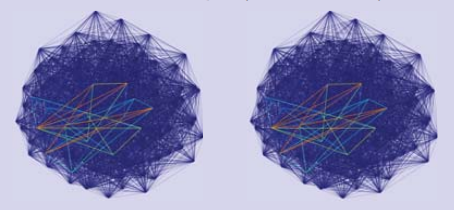
\includegraphics[width=0.8\textwidth]{../img/isomorphism}
    \end{center}
  }
\end{frame}

% TODO: Add some quizzes from the website

\section{Coloring and Connectivity}

\begin{frame}
  \begin{center}
    {\huge
      Graph Coloring
    }
  \end{center}
\end{frame}

\begin{frame}
  \frametitle{Planes and Gates}

  {\larger
    \structure{Graph Coloring} is closely related to
    \alert{Scheduling Problems} 

    \bigskip

    {\bf Example}:
    \begin{itemize}
    \item Every flight requires a \structure{gate} for embark/disembark
    \item Sometimes flight times overlap.
    \item How many gates do we need?
    \end{itemize}
  }

  \hfill 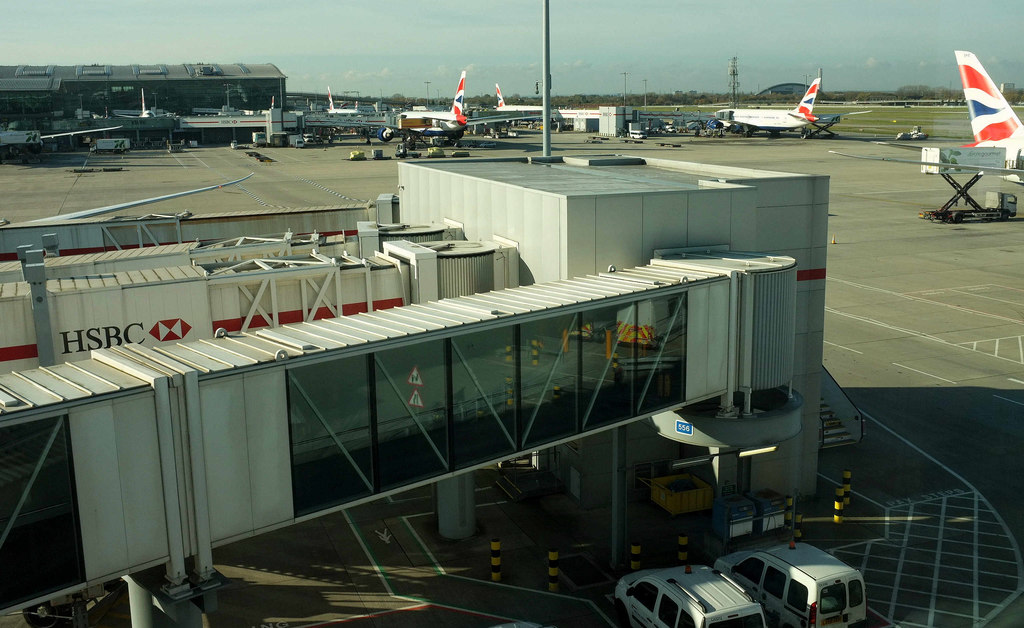
\includegraphics[width=0.5\textwidth]{../img/airgate}
  
\end{frame}

\begin{frame}
  \frametitle{Gate Usage Graph}

  {\larger

    \begin{columns}[T]
      \column{0.7\textwidth}      
      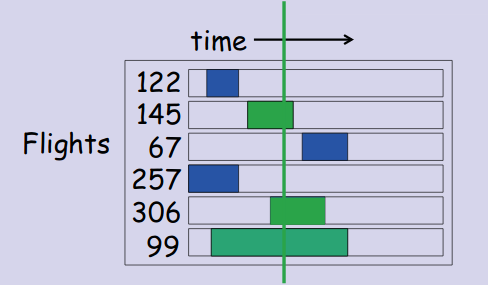
\includegraphics[width=1\textwidth]{../img/gatetable}
      \column{0.3\textwidth}
      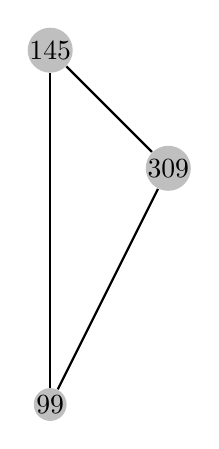
\begin{tikzpicture}[scale=1.5,auto,swap]
        %\tikzset{edge/.style = {->,>=latex'}}
        \node[vertex] (a) at (0,3) {145};
        \node[vertex] (b) at (1,2) {309};
        \node[vertex] (c) at (0,0) {99};
        \draw[edge] (a) to (b);
        \draw[edge] (b) to (c);
        \draw[edge] (c) to (a);
      \end{tikzpicture}

    \end{columns}

    \bigskip
    
    We define a \structure{Gate Usage Graph} where two
    flights are neighbors if \alert{they are on the ground
      at the same time}.
    
  }
\end{frame}

\begin{frame}
  \frametitle{Full Conflict Graph and the Coloring Problem}

  {\large

    \begin{columns}
      \column{0.5\textwidth}
      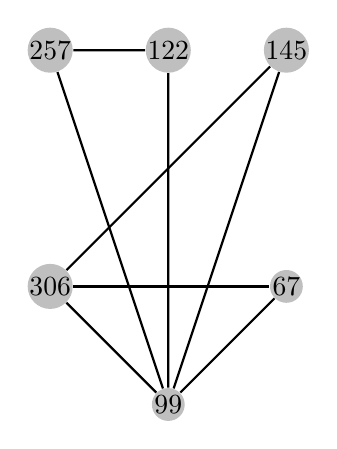
\begin{tikzpicture}[scale=1.5,auto,swap]
        %\tikzset{edge/.style = {->,>=latex'}}
        \node[vertex] (257) at (0,2) {257};
        \node[vertex] (122) at (1,2) {122};
        \node[vertex] (145) at (2,2) {145};
        \node[vertex] (306) at (0,0) {306};
        \node[vertex] (67) at (2,0) {67};
        \node[vertex] (99) at (1,-1) {99};
        \draw[edge] (257) to (122);
        \draw[edge] (257) to (99);
        \draw[edge] (122) to (99);
        \draw[edge] (306) to (99);
        \draw[edge] (67) to (99);
        \draw[edge] (306) to (67);
        \draw[edge] (306) to (145);
        \draw[edge] (145) to (99);
      \end{tikzpicture}
      \column{0.5\textwidth}
      \begin{itemize}
      \item \alert{Color} vertices so that adjacent vertices don't
        have the same color.
      \item If \structure{Edges} = conflict, then \structure{min
        \# colors} = min \# of gates.
      \end{itemize}
    \end{columns}
  }
    
\end{frame}


\begin{frame}
  \frametitle{Full Conflict Graph and the Coloring Problem}

  {\large

    \begin{columns}
      \column{0.5\textwidth}
      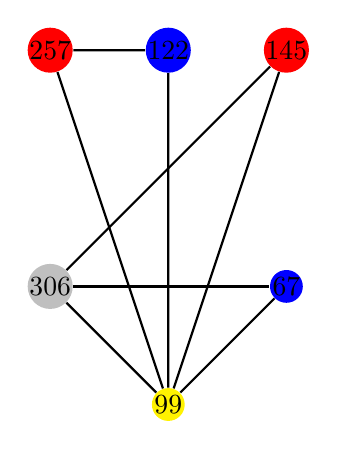
\begin{tikzpicture}[scale=1.5,auto,swap]
        %\tikzset{edge/.style = {->,>=latex'}}
        \node[red vertex] (257) at (0,2) {257};
        \node[blue vertex] (122) at (1,2) {122};
        \node[red vertex] (145) at (2,2) {145};
        \node[vertex] (306) at (0,0) {306};
        \node[blue vertex] (67) at (2,0) {67};
        \node[yellow vertex] (99) at (1,-1) {99};
        \draw[edge] (257) to (122);
        \draw[edge] (257) to (99);
        \draw[edge] (122) to (99);
        \draw[edge] (306) to (99);
        \draw[edge] (67) to (99);
        \draw[edge] (306) to (67);
        \draw[edge] (306) to (145);
        \draw[edge] (145) to (99);
      \end{tikzpicture}
      \column{0.5\textwidth}
      \begin{itemize}
      \item We select colors for each vertex so that no adjacent
        vertex has the same color.

        \bigskip
        
      \item Each color = One new Gate

        \bigskip

      \item Final gate assignment:
        \begin{itemize}
        \item Blue Gate: Flight 122 and 67
        \item Red Gate: Flight 145 and 257
        \item Yellow Gate: Flight 99
        \item Gray Gate: Flight 306
        \end{itemize}

        \bigskip

      \item Can you find a better coloring using
        only \alert{3 gates}?
      \end{itemize}
    \end{columns}
  }
    
\end{frame}

\begin{frame}
  \frametitle{Conflict Allocation Problems}

  {\large

    \begin{columns}
      \column{0.5\textwidth}
      \begin{itemize}
      \item \structure{Allocate classrooms} for courses, when
        courses can be \alert{at the same time}.
        
        \medskip
        
      \item \structure{Allocate cages} for animals, when
        some animals \alert{can not be at the same cage}.
        
        \medskip
        
      \item \structure{Different Frequencies} for radio
        stations, when the radio stations \alert{interfere with
          each other}
        
        \medskip
        
      \item \structure{Map Coloring!}
        
      \end{itemize}

      \column{0.5\textwidth}
      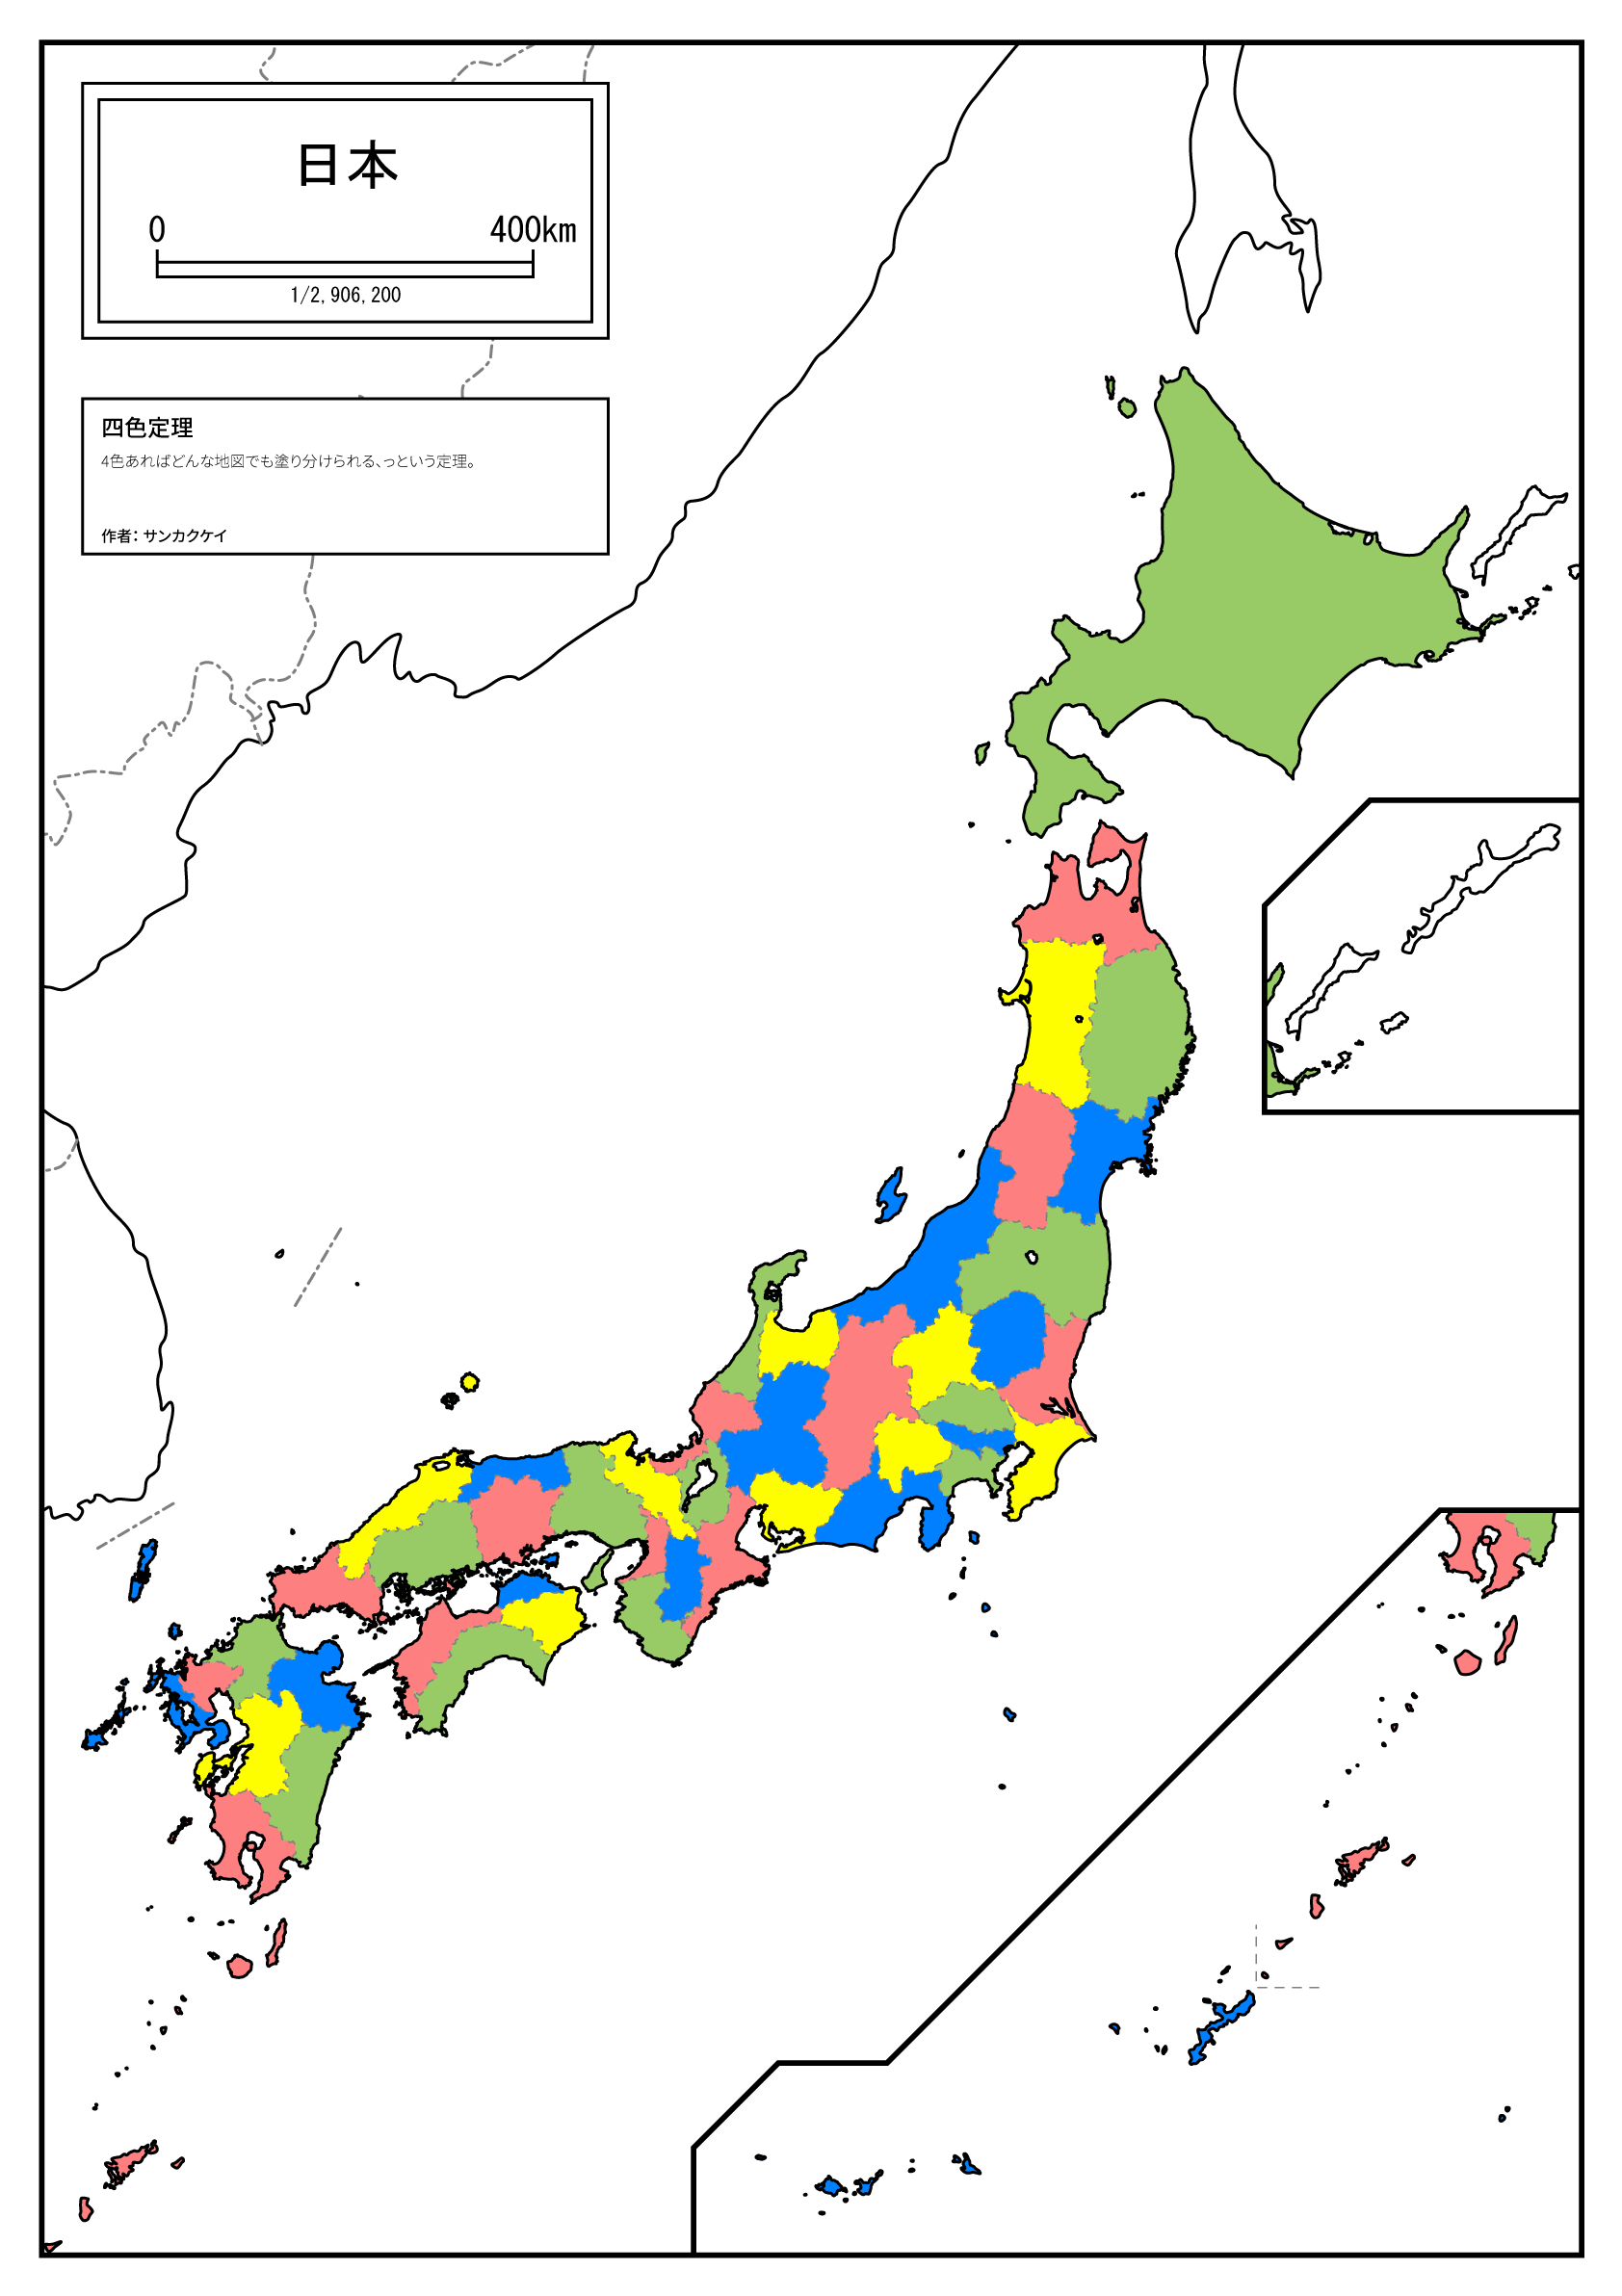
\includegraphics[height=\textheight]{../img/japan4color}
    \end{columns}
  }
\end{frame}

\begin{frame}
  \frametitle{Vertex Coloring and Face Coloring}

  {\larger
    \begin{center}
      Maps to Graphs\\
      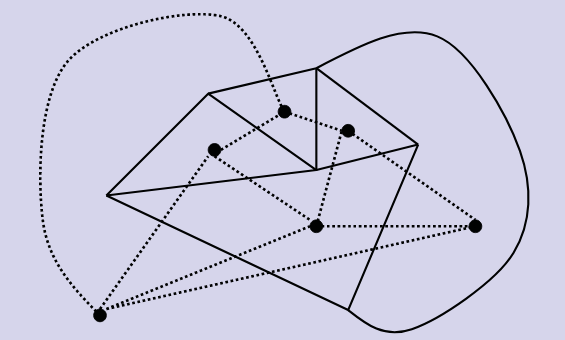
\includegraphics[width=0.6\textwidth]{../img/facecolor}
    \end{center}

    {\bf Theorem:} Maps can always be colored with 4 colors
    \begin{itemize}
    \item 1970: ``Proof'' with computers (checks 1000's of maps)
    \item 1990: Better Mathematical Proof. (still need program)
    \end{itemize}

  }
\end{frame}

\begin{frame}
  \frametitle{Chromatic Number}

  {\larger
    The Chromatic Number $\chi(G)$ is the \structure{minimum} number of
    colors neecessary to color $G$.

    {\bf Examples:}
    \begin{itemize}
    \item Cycle Graphs: $\chi(C_{\text{even}}) = 2$, $\chi(C_{\text{odd}}) = 3$\\
      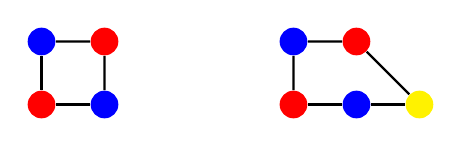
\begin{tikzpicture}[scale=.8,auto,swap]
        %\tikzset{edge/.style = {->,>=latex'}}
        \node[red vertex] (a) at (0,0) {};
        \node[blue vertex] (b) at (1,0) {};
        \node[red vertex] (c) at (1,1) {};
        \node[blue vertex] (d) at (0,1) {};
        \draw[edge] (a) to (b);
        \draw[edge] (b) to (c);
        \draw[edge] (c) to (d);
        \draw[edge] (d) to (a);
        \node[red vertex] (a1) at (4,0) {};
        \node[blue vertex] (b1) at (5,0) {};
        \node[red vertex] (c1) at (5,1) {};
        \node[blue vertex] (d1) at (4,1) {};
        \node[yellow vertex] (e1) at (6,0) {};
        \draw[edge] (a1) to (b1);
        \draw[edge] (b1) to (e1);
        \draw[edge] (e1) to (c1);
        \draw[edge] (c1) to (d1);
        \draw[edge] (d1) to (a1);
      \end{tikzpicture}

    \item Complete Graph with $n$ vertices: $\chi(K_n) = n$\\
      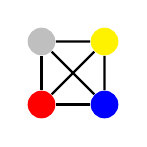
\begin{tikzpicture}[scale=.8,auto,swap]
        %\tikzset{edge/.style = {->,>=latex'}}
        \node[red vertex] (a) at (0,0) {};
        \node[blue vertex] (b) at (1,0) {};
        \node[yellow vertex] (c) at (1,1) {};
        \node[vertex] (d) at (0,1) {};
        \draw[edge] (a) to (b);
        \draw[edge] (b) to (c);
        \draw[edge] (c) to (d);
        \draw[edge] (d) to (a);
        \draw[edge] (a) to (c);
        \draw[edge] (d) to (b);
      \end{tikzpicture}
      
    \item Wheel Graph: $\chi(W_{\text{odd}}) = 4, \chi(W_{\text{even}} = 3)$
      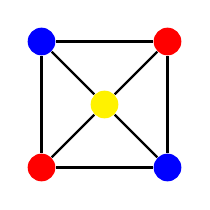
\begin{tikzpicture}[scale=.8,auto,swap]
        %\tikzset{edge/.style = {->,>=latex'}}
        \node[red vertex] (a) at (0,0) {};
        \node[blue vertex] (b) at (2,0) {};
        \node[red vertex] (c) at (2,2) {};
        \node[blue vertex] (d) at (0,2) {};
        \node[yellow vertex] (e) at (1,1) {};
        \draw[edge] (a) to (b);
        \draw[edge] (b) to (c);
        \draw[edge] (c) to (d);
        \draw[edge] (d) to (a);
        \draw[edge] (a) to (e);
        \draw[edge] (b) to (e);
        \draw[edge] (c) to (e);
        \draw[edge] (d) to (e);
      \end{tikzpicture}
    \end{itemize}    
  }
\end{frame}

\begin{frame}
  \frametitle{Bounding Chromatic Numbers}

  {\larger

    \begin{itemize}
    \item All degrees $\leq k \implies \chi(G) \leq k+1$\\
      \hfill (Proof by Greedy coloring algorithm).

      \bigskip

    \item Is the graph 2-colorable?\\
      \hfill ({\bf easy} to check: e.g.: BFS)

      \bigskip
      
    \item Is the graph 3-colorable?\\
      \hfill ({\bf hard} to check)

      \bigskip

    \item Is $\chi(G) = k$?\\
      \hfill (in theory, not harder than 3 color, harder in practice).
      
    \end{itemize}

  }
\end{frame}

\subsection{Connectivity}

\begin{frame}
  \frametitle{Connectivity Definition}

  {\larger
    \begin{itemize}
      
    \item Two vertices are \structure{connected} {\bf iff} there is
      a \structure{path} between the two.
    \item Every vertice is connected to itself.
    \item A whole \structure{graph} is \structure{connected} if
      every vertice is connected to each other.
    \end{itemize}

    \begin{center}
      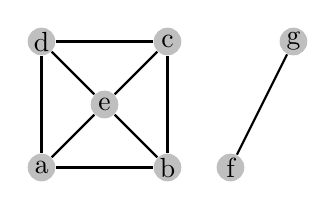
\begin{tikzpicture}[scale=.8,auto,swap]
        %\tikzset{edge/.style = {->,>=latex'}}
        \node[vertex] (a) at (0,0) {a};
        \node[vertex] (b) at (2,0) {b};
        \node[vertex] (c) at (2,2) {c};
        \node[vertex] (d) at (0,2) {d};
        \node[vertex] (e) at (1,1) {e};
        \node[vertex] (f) at (3,0) {f};
        \node[vertex] (g) at (4,2) {g};
        \draw[edge] (a) to (b);
        \draw[edge] (b) to (c);
        \draw[edge] (c) to (d);
        \draw[edge] (d) to (a);
        \draw[edge] (a) to (e);
        \draw[edge] (b) to (e);
        \draw[edge] (c) to (e);
        \draw[edge] (d) to (e);
        \draw[edge] (f) to (g);
      \end{tikzpicture}
    \end{center}
  }
\end{frame}

\begin{frame}
  \frametitle{Connected Components}

  {\larger
    \begin{center}
      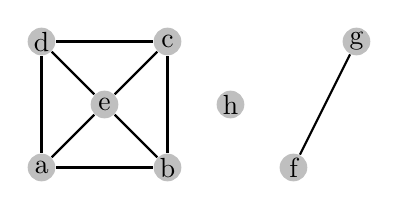
\begin{tikzpicture}[scale=.8,auto,swap]
        %\tikzset{edge/.style = {->,>=latex'}}
        \node[vertex] (a) at (0,0) {a};
        \node[vertex] (b) at (2,0) {b};
        \node[vertex] (c) at (2,2) {c};
        \node[vertex] (d) at (0,2) {d};
        \node[vertex] (e) at (1,1) {e};
        \node[vertex] (f) at (4,0) {f};
        \node[vertex] (g) at (5,2) {g};
        \node[vertex] (h) at (3,1) {h};
        \draw[edge] (a) to (b);
        \draw[edge] (b) to (c);
        \draw[edge] (c) to (d);
        \draw[edge] (d) to (a);
        \draw[edge] (a) to (e);
        \draw[edge] (b) to (e);
        \draw[edge] (c) to (e);
        \draw[edge] (d) to (e);
        \draw[edge] (f) to (g);
      \end{tikzpicture}
    \end{center}

    \begin{itemize}
    \item Every Graph is composed of connected subgraphs called
      \structure{connected~components}
    \item \structure{connected component} of
      v $::=$ \{w | w connected to v\}.
    \item \structure{connected component} of $v = E^*(v)$
      (walk relation of v)

      \bigskip
      
    \item A graph is \structure{connected} {\bf iff} it has exactly 1 connected component.
    \end{itemize}
  }
\end{frame}

\subsection{Color and Connectivity}

\begin{frame}
  \frametitle{Edge connectivity}

  {\larger
    \begin{itemize}
    \item vertices $v,w$ are \structure{k-edge} connected if
      they remain connected whenever \alert{fewer than $k$
        edges are deleted}.

      \begin{center}
      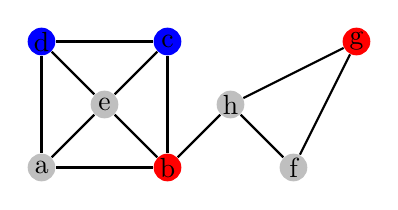
\begin{tikzpicture}[scale=.8,auto,swap]
        %\tikzset{edge/.style = {->,>=latex'}}
        \node[vertex] (a) at (0,0) {a};
        \node[red vertex] (b) at (2,0) {b};
        \node[blue vertex] (c) at (2,2) {c};
        \node[blue vertex] (d) at (0,2) {d};
        \node[vertex] (e) at (1,1) {e};
        \node[vertex] (f) at (4,0) {f};
        \node[red vertex] (g) at (5,2) {g};
        \node[vertex] (h) at (3,1) {h};
        \draw[edge] (a) to (b);
        \draw[edge] (b) to (c);
        \draw[edge] (c) to (d);
        \draw[edge] (d) to (a);
        \draw[edge] (a) to (e);
        \draw[edge] (b) to (e);
        \draw[edge] (c) to (e);
        \draw[edge] (d) to (e);
        \draw[edge] (f) to (g);
        \draw[edge] (f) to (h);
        \draw[edge] (g) to (h);
        \draw[edge] (h) to (b);
      \end{tikzpicture}
    \end{center}

    \item \structure{blue vertices} are 3-edge connected, \alert{red vertices} are 1-edge connected;
    \item A {\bf Graph} is k-edge connected if all pairs of vertices are \structure{at least} k-edge connected.
    \end{itemize}
  }
\end{frame}

\begin{frame}
  \frametitle{Edge Connectivity}

  {\large

    \begin{itemize}
      
    \item {\bf Edge Connectivity} represents the degree of
      {\bf fault tolerance} in a graph.

      
    \item {\bf Example:} In a communication network, how many
      channels can fail before communication is disrupted?

      \bigskip

    \item Related Concept: \structure{k-vertice connectivity}

      \begin{itemize}
      \item k-vertice connected graph $\implies$ k-edge connected;
      \item \alert{BUT!} k-edge connected $\not\implies$ k-vertice
        connected.
      \end{itemize}

    \item The \structure{complete graph} $K_n$ is n-1 connected.      
    \end{itemize}
  }
  
\end{frame}

\begin{frame}
  \frametitle{Connectivity and Hypercubes}

  {\larger

      \begin{center}
      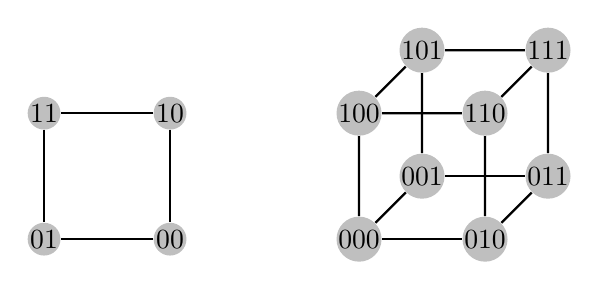
\begin{tikzpicture}[scale=.8,auto,swap]
        %\tikzset{edge/.style = {->,>=latex'}}
        \node[vertex] (00) at (0,0) {00};
        \node[vertex] (01) at (-2,0) {01};
        \node[vertex] (10) at (0,2) {10};
        \node[vertex] (11) at (-2,2) {11};
        \draw[edge] (00) to (10);
        \draw[edge] (10) to (11);
        \draw[edge] (00) to (01);
        \draw[edge] (01) to (11);

        \node[vertex] (000) at (3,0) {000};
        \node[vertex] (010) at (5,0) {010};
        \node[vertex] (100) at (3,2) {100};
        \node[vertex] (110) at (5,2) {110};
        \node[vertex] (001) at (4,1) {001};
        \node[vertex] (011) at (6,1) {011};
        \node[vertex] (101) at (4,3) {101};
        \node[vertex] (111) at (6,3) {111};
        \draw[edge] (000) to (100);
        \draw[edge] (100) to (110);
        \draw[edge] (000) to (010);
        \draw[edge] (010) to (110);
        \draw[edge] (001) to (101);
        \draw[edge] (101) to (111);
        \draw[edge] (001) to (011);
        \draw[edge] (011) to (111);
        \draw[edge] (001) to (000);
        \draw[edge] (111) to (110);
        \draw[edge] (011) to (010);
        \draw[edge] (101) to (100);

        
      \end{tikzpicture}
    \end{center}
    
    \begin{itemize}
    \item Consider the $n$-dimensional hypercube $H_n$
    \item $V(H_n) ::= \{0,1\}^n$
    \item $E(H_n) ::= \{(u,v)$ {\bf iff} u and v differ in 1 bit $\}$

    \item $H_n$ is $n$ vertex connected. ($H_n$ has $n^2$ vertices)
    \end{itemize}

  }
  
\end{frame}

\section{Trees}

\begin{frame}
  \begin{center}
    {\huge Trees}
  \end{center}
\end{frame}

\begin{frame}
  \frametitle{Tree Definitions}

  {\larger
    \begin{itemize}
    \item \structure{Trees} are connected Graphs with \alert{no cycles}.
    \item Has 1-edge connectivity, 1-vertex connectivity.
    \item Chromatic Number = 2

      \bigskip

    \item Trees come up all the time:
      \begin{columns}
        \column{0.5\textwidth}
        \begin{itemize}
        \item Family Trees;
        \item Search Trees;
        \item Game Trees;
        \item Parse Trees;
        \end{itemize}
        \column{0.5\textwidth}
        \begin{itemize}
        \item Spanning Trees;
        \item Rooted Trees;
        \item Ordered Trees;
        \item Binary Trees;
        \item etc...
        \end{itemize}
      \end{columns}
    \end{itemize}
  }
\end{frame}

\begin{frame}
  \frametitle{A few more definitions}

  {\larger
    \begin{itemize}
    \item \structure{Cut Edge}: An edge is a cut edge if
      removing it makes two edges disconnected.

      \bigskip
      
    \item {\bf Lemma:} An edge is not a cut edge if it is on a
      cycle.

      \bigskip
      
    \item A tree is a \structure{connected graph} where
      \structure{every edge is a cut edge}

      \bigskip
      
    \item This implies that a tree is a connected graph which
      is {\bf\structure{Edge Minimal}}
      \begin{itemize}
      \item A tree has the minimum number of edges necessary to
        connect a set of vertices.
      \end{itemize}
    \end{itemize}
  }
\end{frame}

\begin{frame}
  \frametitle{Tree Coloring}

  {\larger
    \begin{itemize}
    \item A tree is a graph with a \structure{unique path}
      between every pair of vertices.

    \item As a consequence, $\chi(\text{tree}) = 2$

    \item {\bf Constructive Demonstration}

      \begin{columns}
        \column{0.7\textwidth}
        \begin{itemize}
        \item Pick any node in the tree to be the {\bf root}, color
          it ``blue''.
        \item Color nodes ``odd'' length from the root as ``red''
        \item Color nodes ``even'' length from the root as ``blue''
        \item This is the algorithm for 2-coloring on general graphs
        \end{itemize}
        \column{0.3\textwidth}

        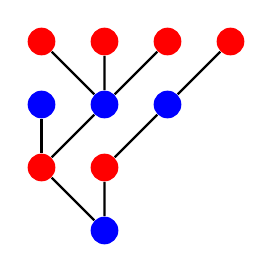
\begin{tikzpicture}[scale=.8,auto,swap]
          %\tikzset{edge/.style = {->,>=latex'}}
          \node[blue vertex] (a) at (1,0) {};
          \node[red vertex] (a1) at (0,1) {};
          \node[red vertex] (b1) at (1,1) {};
          \node[blue vertex] (a2) at (0,2) {};
          \node[blue vertex] (b2) at (1,2) {};
          \node[blue vertex] (c2) at (2,2) {};
          \node[red vertex] (a3) at (0,3) {};
          \node[red vertex] (b3) at (1,3) {};
          \node[red vertex] (c3) at (2,3) {};
          \node[red vertex] (d3) at (3,3) {};          
          \draw[edge] (a) to (a1);
          \draw[edge] (a) to (b1);
          \draw[edge] (a1) to (a2);
          \draw[edge] (a1) to (b2);
          \draw[edge] (b1) to (c2);
          \draw[edge] (b2) to (a3);
          \draw[edge] (b2) to (b3);
          \draw[edge] (b2) to (c3);
          \draw[edge] (c2) to (d3);
          
        \end{tikzpicture}
      \end{columns}
      
    \end{itemize}


    
  }
\end{frame}

\subsection{Spanning Trees}

\begin{frame}
  \frametitle{Spanning Trees}

  {\larger

    \begin{itemize}
    \item A \structure{Spanning Subgraph} of G is a subgraph of
      $G$ that has all vertices of $G$ (and some of the edges).
    \item A \structure{Spanning Tree} of G is a spanning graph of
      $G$ that is also a tree.
    \end{itemize}

    \begin{center}
      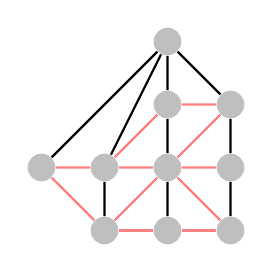
\begin{tikzpicture}[scale=.8,auto,swap]
        %\tikzset{edge/.style = {->,>=latex'}}
        \node[vertex] (a) at (0,1) {};
        \node[vertex] (a1) at (1,0) {};
        \node[vertex] (b1) at (1,1) {};
        \node[vertex] (a2) at (2,0) {};
        \node[vertex] (b2) at (2,1) {};
        \node[vertex] (c2) at (2,2) {};
        \node[vertex] (a3) at (3,0) {};
        \node[vertex] (b3) at (3,1) {};
        \node[vertex] (c3) at (3,2) {};
        \node[vertex] (d3) at (2,3) {};          
        \draw[red edge] (a) to (a1);
        \draw[red edge] (a) to (b1);
        \draw[red edge] (a1) to (a2);
        \draw[red edge] (a1) to (b2);
        \draw[red edge] (b1) to (c2);
        \draw[red edge] (b2) to (a3);
        \draw[red edge] (b2) to (b3);
        \draw[red edge] (b2) to (c3);
        \draw[edge] (c2) to (d3);
        \draw[edge] (a) to (d3);
        \draw[edge] (b1) to (d3);
        \draw[edge] (a1) to (b1);
        \draw[red edge] (b1) to (b2);
        \draw[edge] (b2) to (a2);
        \draw[edge] (b2) to (c2);
        \draw[red edge] (a2) to (a3);
        \draw[red edge] (c2) to (c3);
        \draw[edge] (a3) to (b3);
        \draw[edge] (c3) to (d3);
        \draw[edge] (b3) to (c3);
      \end{tikzpicture}
    \end{center}

    \begin{itemize}
    \item One graph can have multiple spanning trees.
    \item Every connected graph has a spanning tree.
    \end{itemize}    
  }  
\end{frame}

\begin{frame}
  \frametitle{Weighted Spanning Trees}

  {\larger

    The Spanning Tree problem becomes more interesting when we consider
    \structure{weighted edges}.

    \begin{center}
      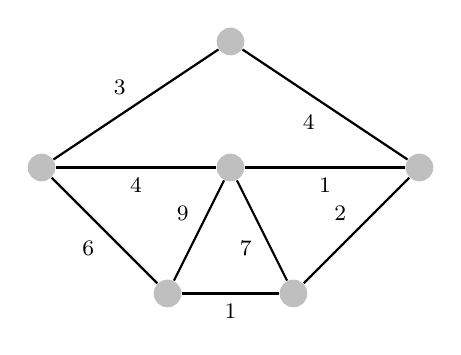
\begin{tikzpicture}[scale=.8,auto,swap]
        %\tikzset{edge/.style = {->,>=latex'}}
        \node[vertex] (a) at (3,5) {};
        \node[vertex] (b) at (0,3) {};
        \node[vertex] (c) at (3,3) {};
        \node[vertex] (d) at (6,3) {};
        \node[vertex] (e) at (2,1) {};
        \node[vertex] (f) at (4,1) {};
        \draw[edge] (a) -- node[weight] {$3$} (b);
        \draw[edge] (a) -- node[weight] {$4$} (d);
        \draw[edge] (b) -- node[weight] {$4$} (c);
        \draw[edge] (c) -- node[weight] {$1$} (d);
        \draw[edge] (b) -- node[weight] {$6$} (e);
        \draw[edge] (c) -- node[weight] {$9$} (e);
        \draw[edge] (c) -- node[weight] {$7$} (f);
        \draw[edge] (d) -- node[weight] {$2$} (f);
        \draw[edge] (e) -- node[weight] {$1$} (f);
      \end{tikzpicture}
    \end{center}

    What is the \structure{minimal cost} structure that
    allows me to connect everything?
    
  }
\end{frame}

\begin{frame}
  \frametitle{Minimum Spanning Tree Algorithm}

  {\larger
    \begin{center}
      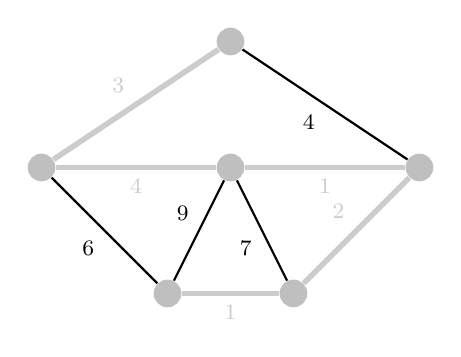
\begin{tikzpicture}[scale=.8,auto,swap]
        %\tikzset{edge/.style = {->,>=latex'}}
        \node[vertex] (a) at (3,5) {};
        \node[vertex] (b) at (0,3) {};
        \node[vertex] (c) at (3,3) {};
        \node[vertex] (d) at (6,3) {};
        \node[vertex] (e) at (2,1) {};
        \node[vertex] (f) at (4,1) {};
        \draw[black edge] (a) -- node[weight] {$3$} (b);
        \draw[edge] (a) -- node[weight] {$4$} (d);
        \draw[black edge] (b) -- node[weight] {$4$} (c);
        \draw[black edge] (c) -- node[weight] {$1$} (d);
        \draw[edge] (b) -- node[weight] {$6$} (e);
        \draw[edge] (c) -- node[weight] {$9$} (e);
        \draw[edge] (c) -- node[weight] {$7$} (f);
        \draw[black edge] (d) -- node[weight] {$2$} (f);
        \draw[black edge] (e) -- node[weight] {$1$} (f);
      \end{tikzpicture}
    \end{center}

    \begin{enumerate}
    \item Start with one arbitrary vertex and add it to the MST.
    \item From all edges connected with the MST, select one with minimum weight;
    \item Add the edge, and vertex, to the MST;
    \item Return to (2)
    \end{enumerate}
  }
\end{frame}

\section{Stable Matching}

\begin{frame}
  \begin{center}
    {\huge
      Stable Matching Problem
    }
  \end{center}
\end{frame}

\begin{frame}
  \frametitle{The Stable Marriage Problem}
  \begin{center}
    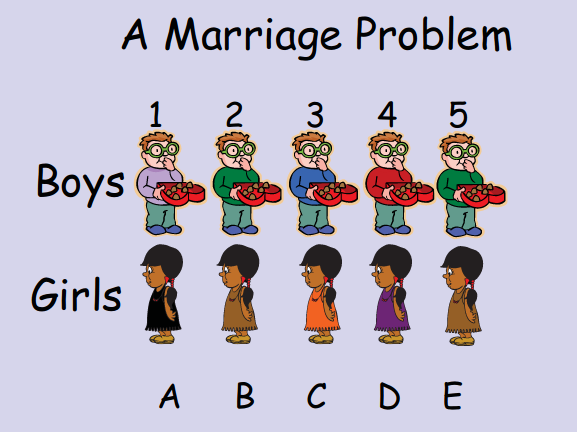
\includegraphics[width=.8\textwidth]{../img/marriage1}
  \end{center}
\end{frame}

\begin{frame}
  \frametitle{Each boy and girl has a preference list}
  \begin{center}
    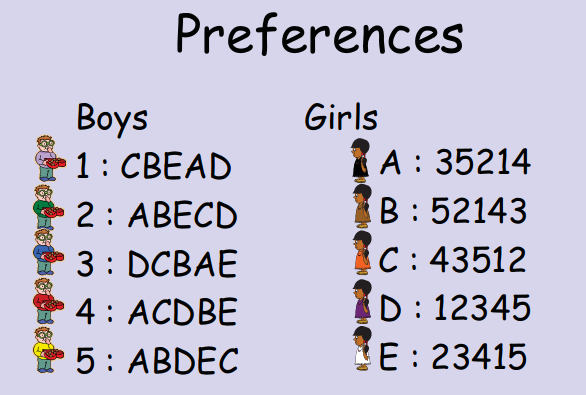
\includegraphics[width=.8\textwidth]{../img/marriage2}
  \end{center}
\end{frame}

\begin{frame}
  \frametitle{``Boy-greedy'' Algorithm}

  {\larger
    Let's marry each boy to their favorite girl:
  }
  \begin{center}
    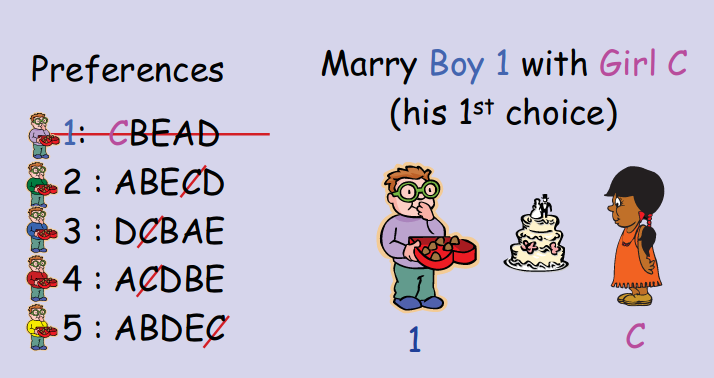
\includegraphics[width=.8\textwidth]{../img/marriage3}
  \end{center}
\end{frame}

\begin{frame}
  \frametitle{``Boy-greedy'' Algorithm}

  {\larger
    Let's marry each boy to their favorite girl:
  }
  \begin{center}
    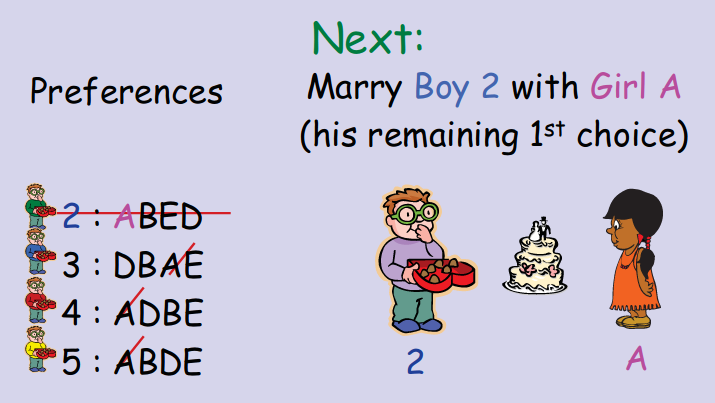
\includegraphics[width=.8\textwidth]{../img/marriage4}
  \end{center}
\end{frame}

\begin{frame}
  \frametitle{``Boy-greedy'' Algorithm}

  {\larger
    Final pairing:
  }
  \begin{center}
    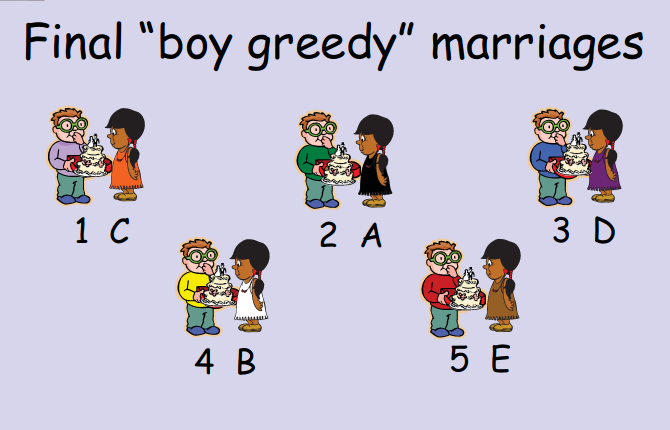
\includegraphics[width=.8\textwidth]{../img/marriage5}
  \end{center}
\end{frame}

\begin{frame}
  \frametitle{Trouble with the boy Greedy algorithm!}
  \begin{center}
    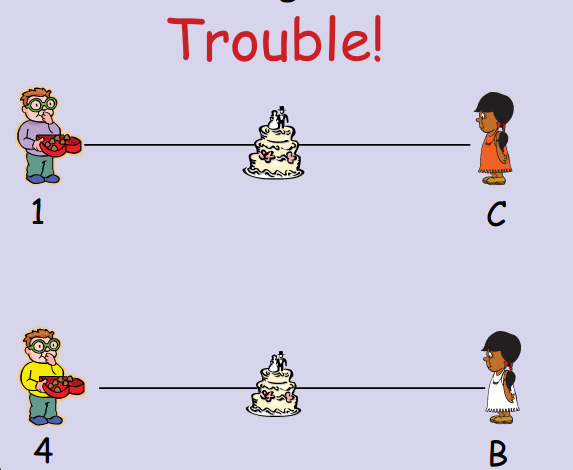
\includegraphics[width=.45\textwidth]{../img/marriage6}
    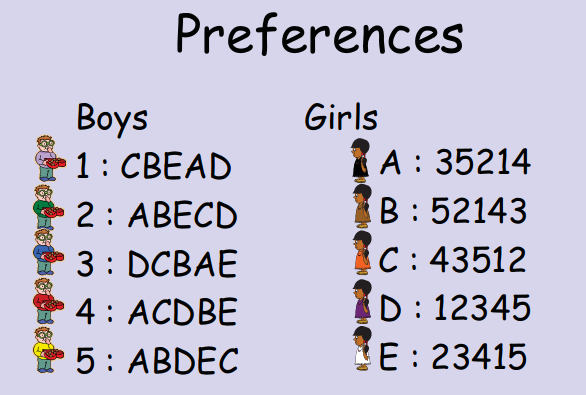
\includegraphics[width=.45\textwidth]{../img/marriage2}
  \end{center}
\end{frame}

\begin{frame}
  \frametitle{Trouble with the boy Greedy algorithm!}

  \begin{center}
    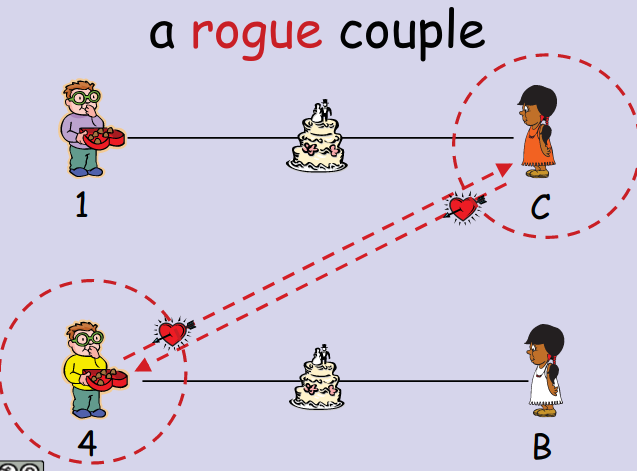
\includegraphics[width=.45\textwidth]{../img/marriage7}
    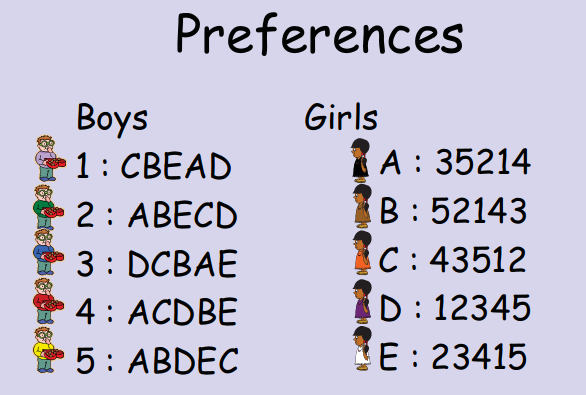
\includegraphics[width=.45\textwidth]{../img/marriage2}
  \end{center}

  {\larger
    \alert{QUIZ:} Find a better pairing!
  }
  
\end{frame}

\begin{frame}
  \frametitle{One stable matching (Girl Greedy)}
  \begin{center}
    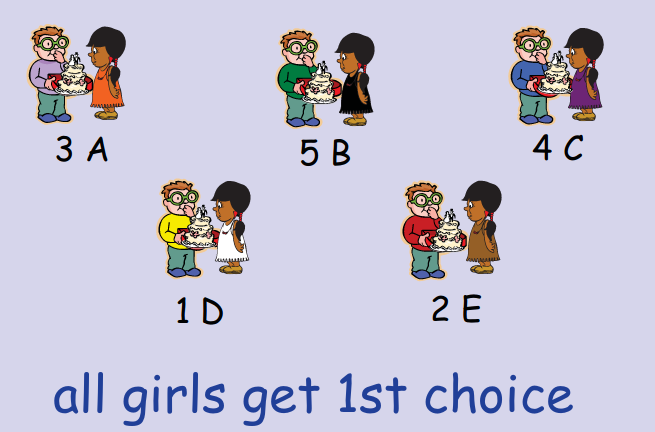
\includegraphics[width=.45\textwidth]{../img/marriage8}
    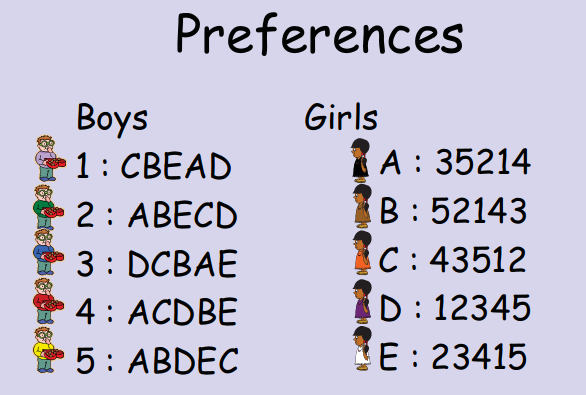
\includegraphics[width=.45\textwidth]{../img/marriage2}
  \end{center}
\end{frame}

\begin{frame}
  \frametitle{Why is the Stable Marriage Problem Important?}

  {\larger
    \begin{itemize}
    \item School Admissions in the US

      \bigskip
      
    \item Matching between Hospitals and Doctors

      \bigskip
      
    \item Akamai Server/Request Matching

      \bigskip
      
    \item Etc...
    \end{itemize}
  }
\end{frame}

\subsection{``Mating Ritual'' Algorithm}

\begin{frame}
  \frametitle{The ``Mating Ritual'' Algorithm}

  {\larger

    Let us describe an algorithm to {\bf always} find a
    stable matching:

    \bigskip

    {\bf Start State:} No boy is proposing to any girl;
    
    \begin{enumerate}
    \item If all girls have $\leq 1$ proposers (and it is
      not the first iteration), they marry and the algorithm stops.
    \item Any girl that has $> 1$ proposers, they reject all except
      the favorite boy.
    \item If any boy is not proposing to anyone, they propose to
      their favorite girl.
    \item Return to (1).
    \end{enumerate}
  }
\end{frame}

\begin{frame}
  \frametitle{Example Execution}

  \begin{columns}
    \column{0.45\textwidth}
    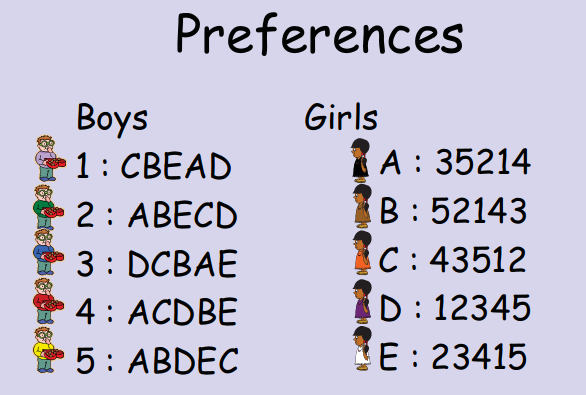
\includegraphics[width=1\textwidth]{../img/marriage2}
    \column{0.55\textwidth}
    {\large
      \begin{itemize}
      \item {\bf iter 1}: No rejections. Proposals:
        \begin{itemize}
        \item A: 2, 4, 5
        \item B:
        \item C: 1
        \item D: 3
        \item E:
        \end{itemize}

      \item {\bf iter 2}: A rejects 2 and 4. Proposals:
        \begin{itemize}
        \item A: 5
        \item B: 2
        \item C: 1, 4
        \item D: 3
        \item E:
        \end{itemize}
      \end{itemize}

    }
  \end{columns}
\end{frame}

\begin{frame}
  \frametitle{Example Execution}

  \begin{columns}
    \column{0.45\textwidth}
    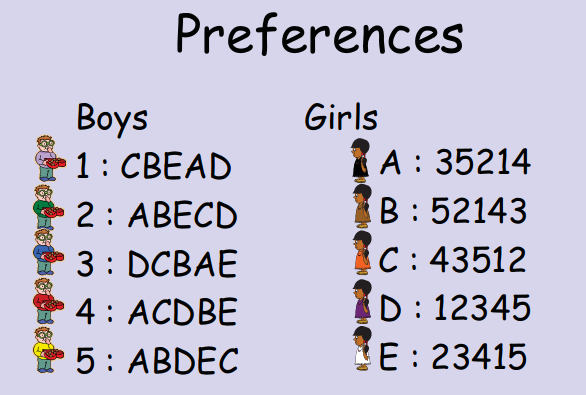
\includegraphics[width=1\textwidth]{../img/marriage2}
    \column{0.55\textwidth}
    {\large
      \begin{itemize}
      \item {\bf iter 3}: C rejects 1. Proposals:
        \begin{itemize}
        \item A: 5
        \item B: 1, 2
        \item C: 4
        \item D: 3
        \item E:
        \end{itemize}

      \item {\bf iter 4}: B rejects 1. Proposals:
        \begin{itemize}
        \item A: 5
        \item B: 2
        \item C: 4
        \item D: 3
        \item E: 1
        \end{itemize}
      \end{itemize}
    }
  \end{columns}
\end{frame}

\begin{frame}
  \frametitle{Proof of Correctness}

  {\larger
    \begin{itemize}
    \item The algorithm stops;
      
      \bigskip

    \item The algorithm is correct when it stops;
    \end{itemize}
  }
\end{frame}

\begin{frame}
  \frametitle{Proof of Correctness: The algorithm stops}

  {\larger
    Every day, the \structure{total number} of girls in
    the boy's lists is reduced.

    \bigskip
    
    \begin{itemize}
    \item The number of girls in the boy's list is reduced
      \structure{when someone is rejected}.
    \item If \structure{no one is rejected} then the algorithm stops.
    \item {\bf Therefore}, every iteration the list of girls reduces
      by at least one.
    \end{itemize}

    \bigskip
    
    Because the total number of girls is \structure{strictly
      decreasing}, the algorithm \alert{must stop}.
  }
\end{frame}

\begin{frame}
  \frametitle{Proof of Correctness: No rogue couples}

  {\larger

    \begin{itemize}
    \item {\bf Lemma 1}: The rank of a girl's favorite is {\bf weakly
      increasing}\\ Every iteration, the girl rejects a favorite {\bf
      iff} she finds a \structure{better one}.

      \bigskip
      
    \item {\bf Lemma 2}: The rank of a boy's favorite is {\bf weakly
      decreating}\\ Every iteration, the boy stays with current
      favorite, or is rejected and goes to the next lower one.
      
    \end{itemize}
  }
\end{frame}

\begin{frame}
  \frametitle{Proof of Correctness: No rogue couples}

  {\larger {\bf Invariant:} If $G_i$ is not on $B_j$ list, she has a
    better curent favorite.

    \bigskip
    
    \begin{itemize}
    \item At the moment that $G_i$ rejected $B_i$, she had a better
      favorite (definition of rejection rule)

      \bigskip

    \item A girl's favorite never get worse (lemma 1)
    \end{itemize}    
  }
\end{frame}

\begin{frame}
  \frametitle{Proof of Correctness: No rogue couples}
  
  {\larger

    {\bf Lemma:} When a Boy $B_i$ marries, he cannot form a rogue
    couple.

    \bigskip

    {\bf Proof by Cases:}
    \begin{itemize}
    \item {\bf Case 1:} $B_i$ tries to form a rogue couple with
      someone not on his list. However, by \alert{Invariant}, any girl
      not on his list has a better favorite, and no rogue couple is
      possible.

    \item {\bf Case 2:} $B_i$ tries to form a rogue couple with
      someone on his list. However, by \alert{Lemma 2}, $B_i$ always
      propose to the best girl in his list, and no rogue couple is
      possible.
    \end{itemize}

    \bigskip

    {\bf Therefore}, no rogue couple is possible.
    
  }
\end{frame}

\section{Conclusion}
\begin{frame}
  \frametitle{Main Points for Today's Class}

  {\larger
    \begin{itemize}
    \item Coloring Problems, and Chromatic Number;

      \bigskip
      
    \item Trees, and Minimum Spanning Tree;

      \bigskip
      
    \item Matching, and the Stable Marriage Problem;
    \end{itemize}
  }
\end{frame}

\begin{frame}
  \frametitle{Extra Topics}

  {\larger

    Check the class materials for ``Hall's Graphs'', for more
    information on matching.
    
  }
  
\end{frame}


\end{document}
